\section{Application: Least squares approximation}

\begin{center}
  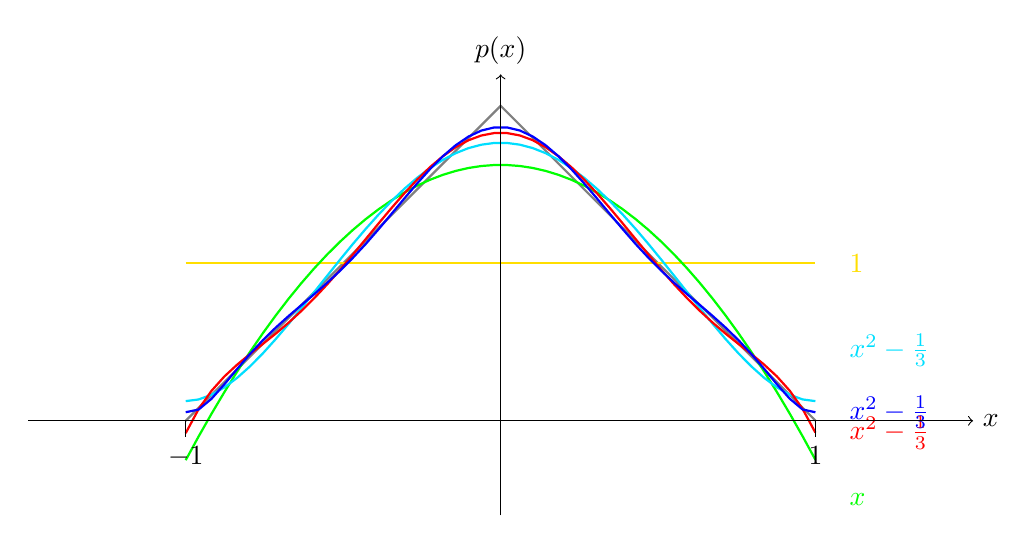
\begin{tikzpicture}[domain=-1:1, scale=4, samples=50]
    \def\fA#1{1}
    \def\fB#1{(#1)}
    \def\fC#1{(abs((#1)^2)-1/3)}
    \def\fD#1{((#1)^3-3/5*(#1))}
    \def\fE#1{(abs((#1)^4)-6/7*abs((#1)^2)+3/35)}
    \def\fF#1{((#1)^5 - 10/9*(#1)^3+5/21*(#1))}
    \def\fG#1{(abs((#1)^6)-15/11*abs((#1)^4)+5/11*abs((#1)^2)-5/231)}
    \def\fH#1{((429*(#1)^7 - 693*(#1)^5 + 315*(#1)^3 - 35*(#1))/429)}
    \def\fI#1{((6435*abs((#1)^8)-12012*abs((#1)^6)+6930*abs((#1)^4)-1260*abs((#1)^2)+35)/6435)}
    \definecolor{my-blue}{rgb}{0,0.87,1.00}
    \definecolor{my-yellow}{rgb}{1.00,0.87,0.00}
    \draw[thick,color=gray] (-1,0) -- (0,1) -- (1,0);
    \draw[thick,color=my-yellow] plot (\x,0.5*\fA{\x}) node[right=2ex] {$1$};
    \draw[thick,color=green] plot (\x,{0.5*\fA{\x} - 0.9375*\fC{\x}}) node[below right=2ex] {$x$};
    \draw[thick,color=my-blue] plot (\x,{0.5*\fA{\x} - 0.9375*\fC{\x} + 0.8203125*\fE{\x}}) node[above right=2ex] {$x^2-\frac{1}{3}$};
    \draw[thick,color=red] plot (\x,{0.5*\fA{\x} - 0.9375*\fC{\x} + 0.8203125*\fE{\x} -1.46630859375*\fG{\x}}) node[right=2ex] {$x^2-\frac{1}{3}$};
    \draw[thick,color=blue] plot (\x,{0.5*\fA{\x} - 0.9375*\fC{\x} + 0.8203125*\fE{\x} -1.46630859375*\fG{\x}+3.338470458984375*\fI{\x}}) node[right=2ex] {$x^2-\frac{1}{3}$};
    \draw[->] (-1.5,0) -- (1.5,0) node[right] {$x$};
    \draw[->] (0,-0.3) -- (0,1.1) node[above] {$p(x)$};
    \draw (1,0) -- (1,-0.05) node[below] {$1$};
    \draw (-1,0) -- (-1,-0.05) node[below] {$-1$};
  \end{tikzpicture}
\end{center}

\begin{center}
  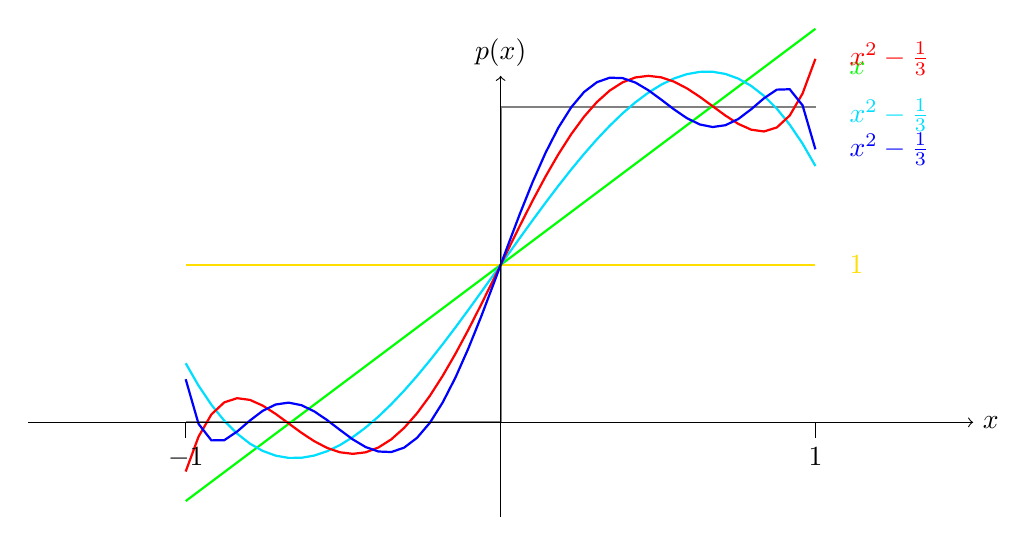
\begin{tikzpicture}[domain=-1:1, scale=4, samples=50]
    \def\fA#1{1}
    \def\fB#1{(#1)}
    \def\fC#1{(abs((#1)^2)-1/3)}
    \def\fD#1{((#1)^3-3/5*(#1))}
    \def\fE#1{(abs((#1)^4)-6/7*abs((#1)^2)+3/35)}
    \def\fF#1{((#1)^5 - 10/9*(#1)^3+5/21*(#1))}
    \def\fG#1{(abs((#1)^6)-15/11*abs((#1)^4)+5/11*abs((#1)^2)-5/231)}
    \def\fH#1{((429*(#1)^7 - 693*(#1)^5 + 315*(#1)^3 - 35*(#1))/429)}
    \def\fI#1{((6435*abs((#1)^8)-12012*abs((#1)^6)+6930*abs((#1)^4)-1260*abs((#1)^2)+35)/6435)}
    \definecolor{my-blue}{rgb}{0,0.87,1.00}
    \definecolor{my-yellow}{rgb}{1.00,0.87,0.00}
    \draw[thick,color=gray] (-1,0) -- (0,0) -- (0,1) -- (1,1);
    \draw[thick,color=my-yellow] plot (\x,0.5*\fA{\x}) node[right=2ex] {$1$};
    \draw[thick,color=green]     plot (\x,{0.5*\fA{\x} + 0.75*\fB{\x}}) node[below right=2ex] {$x$};
    \draw[thick,color=my-blue]   plot (\x,{0.5*\fA{\x} + 0.75*\fB{\x} - 1.09375*\fD{\x}}) node[above right=2ex] {$x^2-\frac{1}{3}$};
    \draw[thick,color=red]       plot (\x,{0.5*\fA{\x} + 0.75*\fB{\x} - 1.09375*\fD{\x} + 2.70703125*\fF{\x}}) node[right=2ex] {$x^2-\frac{1}{3}$};
    \draw[thick,color=blue]      plot (\x,{0.5*\fA{\x} + 0.75*\fB{\x} - 1.09375*\fD{\x} + 2.70703125*\fF{\x} - 7.855224609375*\fH{\x}}) node[right=2ex] {$x^2-\frac{1}{3}$};
    \draw[->] (-1.5,0) -- (1.5,0) node[right] {$x$};
    \draw[->] (0,-0.3) -- (0,1.1) node[above] {$p(x)$};
    \draw (1,0) -- (1,-0.05) node[below] {$1$};
    \draw (-1,0) -- (-1,-0.05) node[below] {$-1$};
  \end{tikzpicture}
\end{center}

\begin{center}
  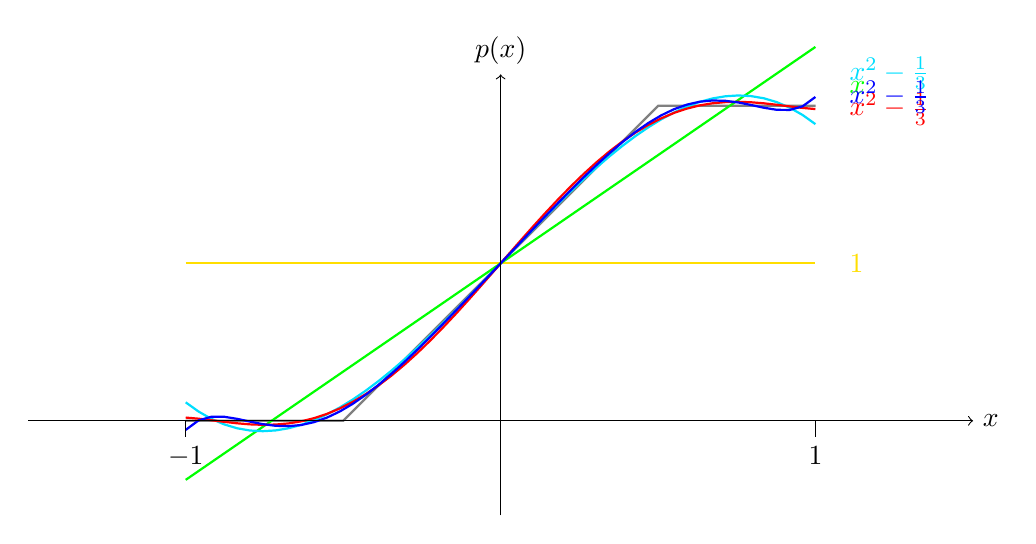
\begin{tikzpicture}[domain=-1:1, scale=4, samples=50]
    \def\fA#1{1}
    \def\fB#1{(#1)}
    \def\fC#1{(abs((#1)^2)-1/3)}
    \def\fD#1{((#1)^3-3/5*(#1))}
    \def\fE#1{(abs((#1)^4)-6/7*abs((#1)^2)+3/35)}
    \def\fF#1{((#1)^5 - 10/9*(#1)^3+5/21*(#1))}
    \def\fG#1{(abs((#1)^6)-15/11*abs((#1)^4)+5/11*abs((#1)^2)-5/231)}
    \def\fH#1{((429*(#1)^7 - 693*(#1)^5 + 315*(#1)^3 - 35*(#1))/429)}
    \def\fI#1{((6435*abs((#1)^8)-12012*abs((#1)^6)+6930*abs((#1)^4)-1260*abs((#1)^2)+35)/6435)}
    \definecolor{my-blue}{rgb}{0,0.87,1.00}
    \definecolor{my-yellow}{rgb}{1.00,0.87,0.00}
    \draw[thick,color=gray] (-1,0) -- (-0.5,0) -- (0.5,1) -- (1,1);
    \draw[thick,color=my-yellow] plot (\x,0.5*\fA{\x}) node[right=2ex] {$1$};
    \draw[thick,color=green]     plot (\x,{0.5*\fA{\x} + 0.6875*\fB{\x}}) node[below right=2ex] {$x$};
    \draw[thick,color=my-blue]   plot (\x,{0.5*\fA{\x} + 0.6875*\fB{\x} - 0.615234375*\fD{\x}}) node[above right=2ex] {$x^2-\frac{1}{3}$};
    \draw[thick,color=red]       plot (\x,{0.5*\fA{\x} + 0.6875*\fB{\x} - 0.615234375*\fD{\x} + 0.38067626953125*\fF{\x}}) node[right=2ex] {$x^2-\frac{1}{3}$};
    \draw[thick,color=blue]      plot (\x,{0.5*\fA{\x} + 0.6875*\fB{\x} - 0.615234375*\fD{\x} + 0.38067626953125*\fF{\x} + 1.0494089126587303*\fH{\x}}) node[right=2ex] {$x^2-\frac{1}{3}$};
    \draw[->] (-1.5,0) -- (1.5,0) node[right] {$x$};
    \draw[->] (0,-0.3) -- (0,1.1) node[above] {$p(x)$};
    \draw (1,0) -- (1,-0.05) node[below] {$1$};
    \draw (-1,0) -- (-1,-0.05) node[below] {$-1$};
  \end{tikzpicture}
\end{center}
